Rozpatrywać będziemy przestrzeń probabilistyczną $(\Omega,\mathcal{F},P)$, czyli niech $\Omega$ to pewien niepusty zbiór, $\mathcal{F}$ to $\sigma$-ciało zdarzeń losowych, a $P$ to funkcja $P\colon\Omega\rightarrow[0,1]$. 

\begin{df}[\textit{n}-wymiarowa zmienna losowa]\cite{Rachunek_prob}
	\label{df:n_wym_zmienna_losowa}
	\textit{n}-wymiarową zmienną losową nazywamy funkcję określoną na przestrzeni zdarzeń elementarnych $\Omega$ i przyjmującą wartości rzeczywiste:
	
	$$ X\colon \Omega \mapsto \mathbb{R}^{n}, $$

	taką, że
	
	$$ \{ \omega \colon X(\omega) < x) \} \in \mathcal{F},$$
	
	dla każdego $x \in \mathbb{R}.$
\end{df}


\subsection{Narzędzia opisu zmiennych losowych}
Zmienna losowa jest matematycznym modelem nieznanej, losowej wielkości. Jest ona jednoznacznie opisywana przez dystrybuantę - mówiącą nam z jakim prawdopodobieństwem zmienna może występować w konkretnych obszarach swojego zbioru wartości.

\begin{df}[Dystrybuanta]\cite{Rachunek_prob}
	Dystrybuantą wektora losowego $\mathbf{X} = [X_1, X_2, \dots, X_n]$ nazywamy funkcję:
	$$
	F_{\mathbf{X}}(x_1, \dots, x_n)=P(X_1 < x_1, \dots, X_n < x_n).
	$$
\end{df}

W tej pracy skupiamy się jedynie na zmiennych losowych typu ciągłego, czyli takich których dystrybuanta daje się przedstawić w postaci $ F_{\mathbf{X}}(x) =\int_{-\infty}^{x}f_{\mathbf{X}}(s) ds$ dla pewnej nieujemnej funkcji $f_{\mathbf{X}(s)}$ nazywanej funkcją gęstości rozkładu. Gęstość, jeżeli jest określona, również może być użyta do jednoznacznej identyfikacji zmiennej losowej.\\

Do opisu najpopularniejszych jednowymiarowych rozkładów dostępne mamy zazwyczaj analityczną postać ich dystrybuanty lub gęstości. Ponieważ literatura podaje różne ich parametryzacje, w tabeli \ref{tab:przykladowe_zmienne_losowe} podajemy gęstości zmiennych losowych przewijających się w tej pracy. Ich wykresy widoczne są na wykresie \ref{fig:przykladowe_zmienne_losowe}. Przykłady wielowymiarowych dystrybuant i gęstości podamy w rozdziale \ref{subsec:rozklady_wielowymiarowe}. 

Warto wspomnieć, że istnieją również użyteczne rozkłady, które nie dają się wyrazić za pomocą gęstości czy dystrybuanty. Najpopularniejszym przykładem mogą być rozkłady stabilne, które w ogólności nie posiadają dystrybuanty jawnej postaci i musimy posługiwać się zamiast tego ich funkcją charakterystyczną. \cite{Stable_Distributions1}, czy \cite{Stable_Distributions2} podają bardzo dobry przegląd teorii rozkładów stabilnych i pokazują ich przewagę w kontekście modelowania nie-gaussowskich zwrotów na rynkach finansowych. \cite{LevyFlights} pokazują natomiast, że modele procesów stochastycznych oparte o rozkład Levy'ego (tzw. \textit{Levy flights}) dobrze nadają się do opisu dynamiki wskaźników finansowych powszechnie używanych w raportach spółek.

\begin{table}[h]
	\caption{\textbf{Popularne zmienne losowe.} Tabela przedstawia dystrybuanty, oraz gęstości popularnych jednowymiarowych zmiennych losowych pojawiających się w tej pracy.}
	\label{tab:przykladowe_zmienne_losowe}
	\begin{tabular}{ll|c|c}
		\hline
		\textbf{Rozkład} & \textbf{Oznaczenie} & \textbf{Nośnik} & \textbf{Gęstość} \\
		\hline
		Normalny & $\mathcal{N}(\mu, \sigma)$ & $\mathbb{R}$ & $\frac{1}{\sigma \sqrt{2 \pi}} \exp\big(-\frac{(x-\mu)^2}{2\sigma^2}\big)$\\ 
		T-studenta & $\text{t}(\mu, \sigma, \nu)$ & $\mathbb{R}$ & $ \frac{\Gamma(\frac{\nu + 1}{2})}{\Gamma(\frac{\nu}{2})\sqrt{\pi\nu}\sigma} \bigg[1 + \big(\frac{x - \mu}{\sigma}\big)^2\frac{1}{\nu}\bigg]^{-\frac{\nu + 1}{2}} $ \\ 
		Beta & $\text{Beta}(\alpha, \beta)$ & $[0, 1]$ & $ x^{\alpha - 1}(1 - x)^{\beta - 1}\frac{\Gamma(\alpha + \beta)}{\Gamma(\alpha)\Gamma(\beta)}$ \\ 
		Wykładniczy & $\text{Exp}(\lambda)$ & $\mathbb{R}^{+}$ & $ \lambda e^{-\lambda x}$ \\
		Gamma & $\mathcal{G}(\alpha, \beta)$ & $\mathbb{R}^+$ & $x^{\alpha - 1}e^{-\beta x}\frac{\beta^\alpha}{\Gamma(\alpha)}$\\ 
		
		\hline
	\end{tabular}
\end{table}

\begin{figure}[H]
	\centering
	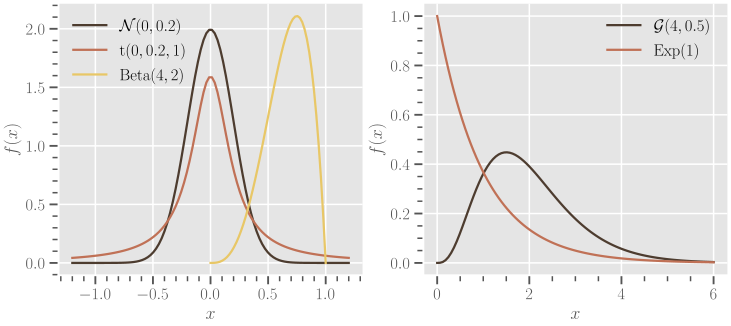
\includegraphics[width=0.8\linewidth]{01_Rozklady_1D}
	\caption{Przykładowe gęstości zmiennych losowych z tabeli \ref{tab:przykladowe_zmienne_losowe}.\label{fig:przykladowe_zmienne_losowe}}
\end{figure}

\subsection{Rozkłady wielowymiarowe}

W klasycznym studium doboru struktury portfela przedstawionym w \cite{Markovitz_MPT}, Markovitz analizuje portfel aktywów. Przedmiotem tej pracy jest opis sposobu, w jaki indywidualne pozycje w portfelu wpływają na jego całościowy zwrot i ryzyko. Współczesna teoria portfela która została zapoczątkowana tą pracą wymaga zamodelowania całego systemu jakim jest zbiór akcji w portfelu. Markovitz pokazuje w swojej pracy istotę współzależności między poszczególnymi aktywami, od której zależy czy ryzyko portfela ulega dywersyfikacji, czy jest amplifikowane. Modelowanie każdego aktywa z osobna jest niewystarczające, ponieważ istota ich wpływu na portfel tkwi w przeważającym stopniu we współzależnościach pomiędzy nimi.\\
Naturalnym jest więc, że w praktyce rozważamy modele wielowymiarowych zmiennych losowych, które mają w sobie zakodowane współzależności i pozwalają przez to lepiej uchwycić losową naturę zjawiska. Z tego samego powodu jednak, rozkłady wielowymiarowe są dużo trudniejsze do modelowania niż ich jednowymiarowe odpowiedniki. Nie wystarczy bowiem zamodelować rozkładów konkretnych współrzędnych wielowymiarowego wektora, lecz należy dodatkowo określić w jaki sposób rozkład tej zmiennej będzie wyglądał, gdy pozostałe zmienne przyjmą wartości w pewnym zbiorze. Odpowiedzi na te pytania dostarczają nam gęstości brzegowe i warunkowe wielowymiarowego rozkładu.
\begin{df}[Rozkłady brzegowy]
	Rozpatrzmy d-wymiarową zmienną losową $\mathbf{X} = [X_1, X_2, \dots, X_d]$ o gęstości $f(x_1, \dots, x_d)$. Gęstość rozkładu brzegowego $f_{j}(x_j)$ definiujemy jako:
	$$f_j(x_j)=\int_{-\infty}^{\infty}\dots\int_{-\infty}^{\infty} f(x_1, \dots, x_{j-1}, x, x_{j+1}, \dots, x_d)  dx_1\dots dx_{j-1} dx_{j+1} \dots dx_d.$$
\end{df}

\begin{df}[Rozkład warunkowy]
	Rozpatrzmy d-wymiarową zmienną losową $\mathbf{X} = [X_1, X_2, \dots, X_d]$ o gęstości $f(x_1, \dots, x_d)$. Gęstość rozkładu warunkowego definiujemy jako:
	 $$f_{j|k}(x_j|x_k) = \frac{f(x_1, \dots, x_d)}{f_k(x_k)}.$$
\end{df}

Rozkłady jednowymiarowe z tabeli \ref{tab:przykladowe_zmienne_losowe} w naturalny sposób znajdują swoje rozszerzenia na więcej wymiarów (\cite{MultivariateDistributions}, \cite{Cherubini_Copula_Methods_in_Finance}). Najpopularniejszym tego przykładem jest rodzina $d$-wymiarowych rozkładów eliptycznych, do której należą rozkłady o gęstości postaci:

$$ f_{\mathcal{N}}(x, \mu, \Sigma) = k_d \vert\Sigma\vert^{-0.5}g\big((x-\mu)^T\Sigma^{-1}(x-\mu)\big).$$

W powyższej reprezentacji, $k_d \in\mathbb{R}$ jest stałą zależną od wymiaru, $\mu$ jest $d$-wymiarowym wektorem średnich, $\Sigma \in \mathbb{R}^{d \times d}$ to symetryczna, dodatnio zdefiniowana macierz, a $g \colon [0, \infty) \mapsto [0, \infty)$ jest pewną funkcją która nie zależy od wymiaru wektora.

Dla odpowiednio dobranych $g$ i $k_d$ otrzymamy w tej rodzinie wielowymiarowy rozkład normalny, czy wielowymiarowy rozkład t. Powstają one przy odpowiednio $k_d=(2\pi)^{-0.5d}$ i $g(s) = \exp(-0.5 t)$, lub $k_d=\Gamma(\frac{\nu + d}{2})/\Gamma(\frac{\nu}{2})$ i $g(s) = \big(1 + \frac{t}{\nu})^{-(\nu + d)/2}$ (Rysunek \ref{fig:multivariate_gaussian_student}).
\begin{figure}[H]
	\centering
	\includegraphics[width=0.8\linewidth]{01_MultivariateGaussianStudent}
	\caption{Rozkłady eliptyczne ($d=2, \mu=[0, 0], \Sigma = \big[\begin{smallmatrix}2&1\\1&2\end{smallmatrix}\big]$). Lewy panel: $2$-wymiarowy rozkład normalny. Prawy panel: $2$-wymiarowy rozkład t ($\nu = 0.5$).\label{fig:multivariate_gaussian_student}}
\end{figure}

W powyższych przykładach należy zaznaczyć, że użycie rodziny rozkładów eliptycznych implikuje rodziny wszystkich rozkładów brzegowych (wielowymiarowy rozkład normalny daje normalne rozkłady brzegowe, wielowymiarowy rozkład $t$ daje rozkłady brzegowe $t$, itd.). Manipulując rozkładami eliptycznymi możemy zamodelować szeroką gamę korelacji między zmiennymi, czy też modelować ich ciężkie ogony zachowując prostotę i analityczną postać modelu. \cite{Markovitz_MPT} i jego model bazują właśnie na rozkładzie multinormalnym, co można uznać za nierealistyczne i oderwane od rzeczywistości ze względu na ciężkoogonowy charakter zwrótów na rynku akcji. Nie mniej jednak nie da się odmówić, że ten prosty model jest wystarczający aby zilustrować jak istotny jest wpływ zależności komponentów na zachowanie całego systemu. \\
Na szczęście dzięki \cite{Sklar_Theorem}, dostepne mamy narzędzia pozwalające uchwycić te zależności dużo dokładniej i \cite{Cherubini_Copula_Methods_in_Finance} czy \cite{Kurowicka_Dependence_Modeling} słusznie wymieniają wiele realnych przykładów gdzie taki wyższy poziom elastyczności modelu jest niezastąpiony. Kolejny rozdział rozpoczniemy od jednego z takich przykładów, w celu umotywowania popularności modeli kopułowych jako odpowiedzi na te potrzeby.